%%%%%%%%%%%%%%%%%%%%%%%%%%%%%%%%%%%%%%%%%
% Journal Article
% LaTeX Template
% Version 1.4 (15/5/16)
%
% This template has been downloaded from:
% http://www.LaTeXTemplates.com
%
% Original author:
% Frits Wenneker (http://www.howtotex.com) with extensive modifications by
% Vel (vel@LaTeXTemplates.com)
%
% License:
% CC BY-NC-SA 3.0 (http://creativecommons.org/licenses/by-nc-sa/3.0/)
%
%%%%%%%%%%%%%%%%%%%%%%%%%%%%%%%%%%%%%%%%%

%----------------------------------------------------------------------------------------
%	PACKAGES AND OTHER DOCUMENT CONFIGURATIONS
%----------------------------------------------------------------------------------------

\documentclass[twoside,twocolumn]{article}

\usepackage{blindtext} % Package to generate dummy text throughout this template 

\usepackage{hyperref}
\hypersetup{
    colorlinks=true,
    linkcolor=blue,
    filecolor=magenta,      
    urlcolor=cyan,
}

\usepackage[sc]{mathpazo} % Use the Palatino font
\usepackage[T1]{fontenc} % Use 8-bit encoding that has 256 glyphs
\linespread{1.05} % Line spacing - Palatino needs more space between lines
\usepackage{microtype} % Slightly tweak font spacing for aesthetics
\usepackage[utf8]{inputenc}

\usepackage[portuguese]{babel} % Language hyphenation and typographical rules

\usepackage[hmarginratio=1:1,top=32mm,columnsep=20pt]{geometry} % Document margins
\usepackage[hang, small,labelfont=bf,up,textfont=it,up]{caption} % Custom captions under/above floats in tables or figures
\usepackage{booktabs} % Horizontal rules in tables

\usepackage{lettrine} % The lettrine is the first enlarged letter at the beginning of the text
\usepackage{float}
\usepackage{enumitem} % Customized lists
\setlist[itemize]{noitemsep} % Make itemize lists more compact

\usepackage{abstract} % Allows abstract customization
\renewcommand{\abstractnamefont}{\normalfont\bfseries} % Set the "Abstract" text to bold
\renewcommand{\abstracttextfont}{\normalfont\small\itshape} % Set the abstract itself to small italic text
%\usepackage[shortlabels]{enumitem}
\usepackage{enumitem}
\usepackage{titlesec} % Allows customization of titles
\renewcommand\thesection{\Roman{section}} % Roman numerals for the sections
\renewcommand\thesubsection{\roman{subsection}} % roman numerals for subsections
\titleformat{\section}[block]{\large\scshape\centering}{\thesection.}{1em}{} % Change the look of the section titles
\titleformat{\subsection}[block]{\large}{\thesubsection.}{1em}{} % Change the look of the section titles

\usepackage{fancyhdr} % Headers and footers
\pagestyle{fancy} % All pages have headers and footers
\fancyhead{} % Blank out the default header
\fancyfoot{} % Blank out the default footer
\fancyhead[C]{MO443 $\bullet$ Abril 2019 $\bullet$ Relatório 01} % Custom header text
\fancyfoot[RO,LE]{\thepage} % Custom footer text

\usepackage{titling} % Customizing the title section

\usepackage{hyperref} % For hyperlinks in the PDF

\usepackage{graphicx}
\usepackage{subfigure}

\usepackage{mathtools}
\DeclarePairedDelimiter\floor{\lfloor}{\rfloor}
%----------------------------------------------------------------------------------------
%	TITLE SECTION
%----------------------------------------------------------------------------------------

\setlength{\droptitle}{-4\baselineskip} % Move the title up

\pretitle{\begin{center}\Huge\bfseries} % Article title formatting
\posttitle{\end{center}} % Article title closing formatting
\title{Relatório - Trabalho 01 \\ \Large MO443 - Introdução ao Processamento de Imagem Digital} %
%\subtitle{qsdqwdqwd} %Article title
\author{%
\textsc{Vinicius Teixeira de Melo - RA: 230223} \\[1ex] % Your name
\normalsize Universidade Estadual de Campinas \\ % Your institution
\normalsize \href{mailto:viniciusteixeira@liv.ic.unicamp.br}{viniciusteixeira@liv.ic.unicamp.br} % Your email address
%\and % Uncomment if 2 authors are required, duplicate these 4 lines if more
%\textsc{Jane Smith}\thanks{Corresponding author} \\[1ex] % Second author's name
%\normalsize University of Utah \\ % Second author's institution
%\normalsize \href{mailto:jane@smith.com}{jane@smith.com} % Second author's email address
}
\date{\today} % Leave empty to omit a date
\renewcommand{\maketitlehookd}{%
%\begin{abstract}
%\noindent \blindtext % Dummy abstract text - replace \blindtext with your abstract text
%\end{abstract}
}

%----------------------------------------------------------------------------------------

\begin{document}

% Print the title
\maketitle

%----------------------------------------------------------------------------------------
%	ARTICLE CONTENTS
%----------------------------------------------------------------------------------------

\section{Especificação do Problema}

O objetivo deste trabalho é implementar alguns filtros de imagens no domínio espacial e de frequências. A filtragem aplicada a uma imagem digital é uma operação local que altera os valores de intensidade dos pixels da imagem levando-se em conta tanto o valor do pixel em questão quanto valores de pixels vizinhos.

No processo de filtragem, utiliza-se uma operação de convolução de uma máscara pela imagem. Este processo equivale a percorrer toda a imagem alterando seus valores conforme os pesos da máscara e as intensidades da imagem.

O trabalho está dividido em duas seções principais:

\begin{itemize}
	\item Filtragem no Domínio Espacial
	\item Filtragem no Domínio de Frequências
\end{itemize}

Na seção de filtragem no domínio espacial, são dados 4 seguintes tipos de filtros:

\begin{enumerate}[label=(\alph*)]
\item $h_{1} = $ \begin{tabular}[H]{|c|c|c|c|c|}
\hline
0  & 0  & -1 & 0  & 0  \\ \hline
0  & -1 & -2 & -1 & 0  \\ \hline
-1 & -2 & 16 & -2 & -1 \\ \hline
0  & -1 & -2 & -1 & 0  \\ \hline
0  & 0  & -1 & 0  & 0  \\ \hline
\end{tabular}

\item $h_{2} = \frac{1}{256}$ \begin{tabular}{|c|c|c|c|c|}
\hline
1 & 4  & 6  & 4  & 1 \\ \hline
4 & 16 & 24 & 16 & 4 \\ \hline
6 & 24 & 36 & 24 & 6 \\ \hline
4 & 16 & 24 & 16 & 4 \\ \hline
1 & 4  & 6  & 4  & 1 \\ \hline
\end{tabular}

\item $h_{3} = $ \begin{tabular}{|c|c|c|}
\hline
-1 & 0 & 1 \\ \hline
-2 & 0 & 2 \\ \hline
-1 & 0 & 1 \\ \hline
\end{tabular}

\item $h_{4} = $ \begin{tabular}{|c|c|c|}
\hline
-1 & -2 & -1 \\ \hline
0  & 0  & 0  \\ \hline
1  & 2  & 1  \\ \hline
\end{tabular}
\end{enumerate}

As aplicações dos filtros devem ser feitas de forma individual, porém, os filtros $h_{3}$ e $h_{4}$ devem ser aplicados de forma combinada, somando-se as respostas de cada um dos filtros por meio da seguinte expressão: $\sqrt{(h_{3})^{2} + (h_{4}})^{2}$.

Na seção de filtragem no domínio de frequências, é necessário aplicar um filtro Gaussiano em uma imagem representada por seu espectro de Fourier, e a componente de frequência zero deve ser transladada para o centro do espectro. Nesse experimento, é necessário testar diferentes graus de suavização, de forma a borrar a imagem com mais ou menos intensidade.

%------------------------------------------------

\section{Entrada de Dados}

O código fonte criado para a execução de todas as tarefas está no notebook \textbf{Trabalho 01.ipynb}. O código foi criado para aceitar imagens em tons de cinza no formato RGB (\textit{Red, Green and Blue}) do tipo PNG (\textit{Portable Network Graphics}).

Para executar o notebook, basta iniciar o ambiente \textit{Jupyter Notebook}, abrir o notebook \textbf{Trabalho 01.ipynb} e executar as células em ordem. Todo o algoritmo foi implementado na linguagem Python na versão 3.6.

As imagens de entrada utilizadas nos testes do algoritmo foram retiradas da página do prof. Hélio Pedrini: \href{http://www.ic.unicamp.br/~helio/imagens_png/}{Imagens}. Na pasta \textbf{imgs/} estão as duas imagens monocromáticas utilizadas nos testes: \textbf{baboon.png} e \textbf{butterfly.png}. As dimensões das imagens de entrada utilizadas são 512x512.

\begin{figure}[tb]
\begin{center}
	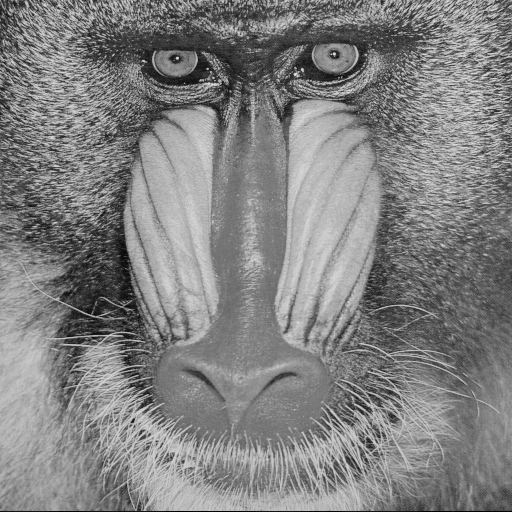
\includegraphics[height=5cm]{figures/baboon.png}
\caption{baboon.png} \label{gdimotes}
\end{center}
\end{figure}

\begin{figure}[tb]
\begin{center}
	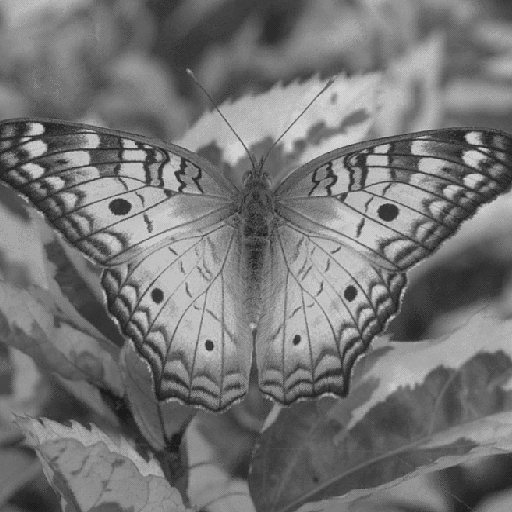
\includegraphics[height=5cm]{figures/butterfly.png}
\caption{butterfly.png} \label{gdimotes}
\end{center}
\end{figure}

%------------------------------------------------

\section{Dependências e Códigos}

As bibliotecas utilizadas neste trabalho foram:

\begin{table}[H]
\begin{tabular}{|l|l|}
\hline
\textbf{Biblioteca} & \textbf{Versão} \\ \hline
numpy               & 1.16.2          \\ \hline
cv2                 & 3.4.2           \\ \hline
matplotlib          & 3.0.3           \\ \hline
skimage             & 0.15.0          \\ \hline
scipy               & 1.2.1           \\ \hline
warnings            & 2.1             \\ \hline
\end{tabular}
\end{table}

A leitura das imagens foi realizada utilizando uma função do \textbf{opencv} \cite{b1} chamada \textbf{imread()}, a qual necessitou de uma constante do próprio \textbf{opencv} para que a imagem ficassem apenas com o canal de escala de cinza, essa constante é denominada \textbf{IMREAD\_GRAYSCALE}.

Os filtros foram gerados manualmente através da função \textbf{numpy.array()}. A função para gerar o preenchimento de borda presente no código utiliza uma função pronta do \textbf{opencv} denominada \textbf{copyMakeBorder()}, a qual preenche na largura a na altura a imagem com valor de \textit{pixel} 0.

A função de convolução 2D foi criada manualmente, mas antes de acontecer as multiplicações e somas, o filtro sofre uma rotação de $180^{\circ}$ utilizando a função \textbf{numpy.rot90()} duas vezes. Para plotar os resultados utilizamos a biblioteca \textbf{matplotlib}.

Para o cálculo da última questão da \textbf{seção 1.1}, foi necessário transformar a saída da aplicação do filtro $h_{3}$ e $h_{4}$ em inteiros de 32 \textit{bits}, pois na expressão $\sqrt{(h_{3})^{2} + (h_{4}})^{2}$ pode haver um estouro de inteiro, por conta de estar representado, inicialmente, por inteiros de 8 \textit{bits}.

Na \textbf{seção 1.2} são utilizadas as funções \textbf{cv2.dft()} e \textbf{cv2.idft()} para transformação de Fourier e transformação inversa de Fourier, respectivamente. Após levar a imagem para o domínio de frequência é necessário transladar a componente de frequência zero para o centro da imagem, para isso é utilizado a função \textbf{numpyp.fft.fftshift()} e, para ter essa operação inversa, é utilizado a função \textbf{numpy.fft.ifftshift()}.

%------------------------------------------------

\section{Fundamentação}

\subsection{Preenchimento de borda}

As imagens de entrada foram carregadas em memória utilizando uma função do \textbf{OpenCv} \cite{b1} que lê a imagem em escala de cinza e salva em uma estrutura $I_{m x n}$, na qual $m$ e $n$ representa a largura e a altura da imagem, respectivamente.

Para a aplicação da operação de convolução na imagem, foi necessário realizar um pré-processamento chamado de \textit{padding}. A operação de \textit{padding} é usada para gerar espaços em torno do conteúdo de um elemento, nesse caso, a imagem. Nesse trabalho, o \textit{padding} gerado nas imagens foi de tamanho $\floor*{\frac{x}{2}}$, onde $x$ é a dimensão do filtro que será convoluído com a imagem. Todo o \textit{padding} foi preenchido com o valor $0$, ou seja, com a cor preta.

\subsection{Convolução 2D}

Convolução 2D é uma operação que, a partir de imagem e um filtro, resulta em uma terceira imagem que mede a soma do produto da imagem e o filtro inicial ao longo da região subentendida pela superposição delas em função do deslocamento existente entre elas.

\begin{figure}[H]
\begin{center}
	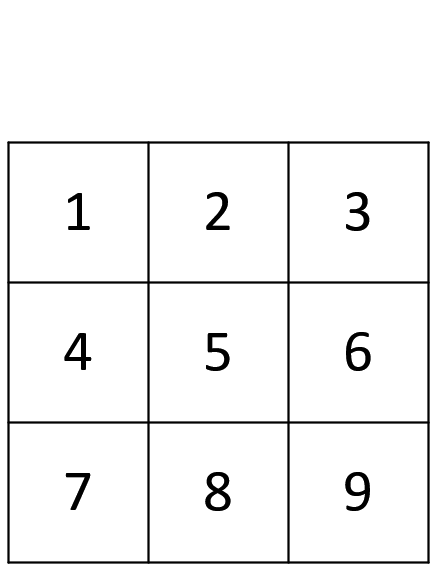
\includegraphics[scale=.2]{figures/entrada.png}
	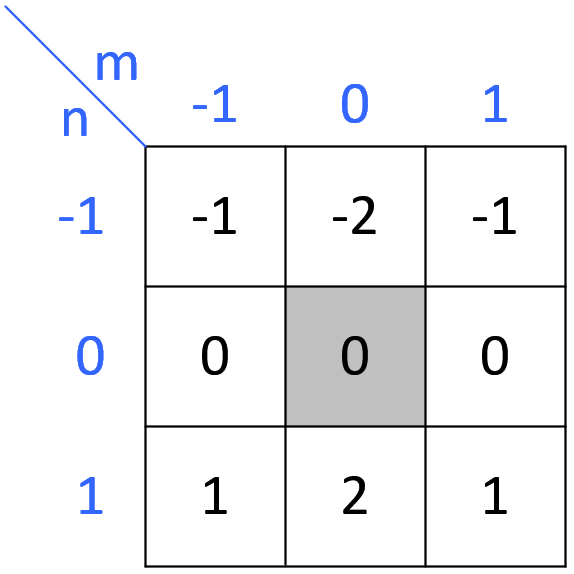
\includegraphics[scale=.2]{figures/filtro.png}
	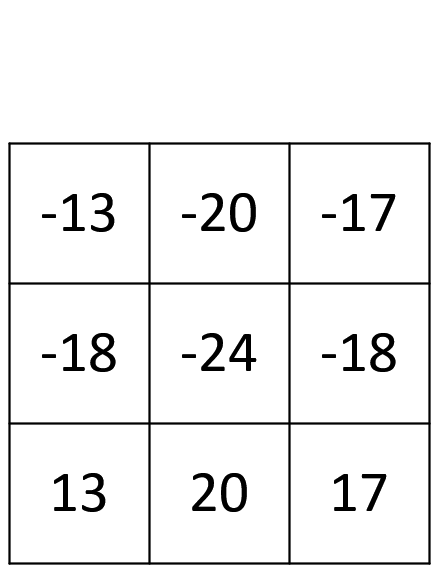
\includegraphics[scale=.2]{figures/resultado.png}
\caption{Exemplo de imagem, filtro e resultado da convolução, respectivamente.} \label{gdimotes}
\end{center}
\end{figure}

A operação de convolução, primeiramente, rotaciona o filtro em $180^{\circ}$ e depois multiplica \textit{pixel} a \textit{pixel}, da seguinte forma:

\begin{figure}[H]
\begin{center}
	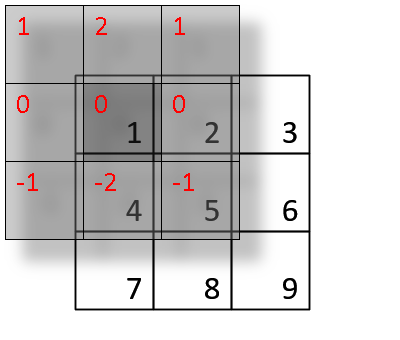
\includegraphics[scale=.2]{figures/mult1.png}
	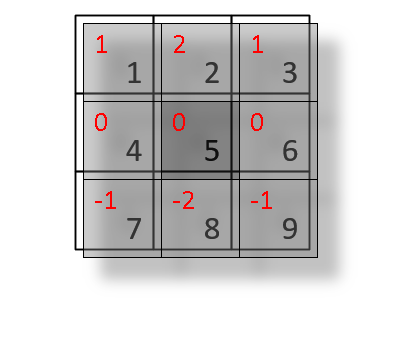
\includegraphics[scale=.2]{figures/multi5.png}
	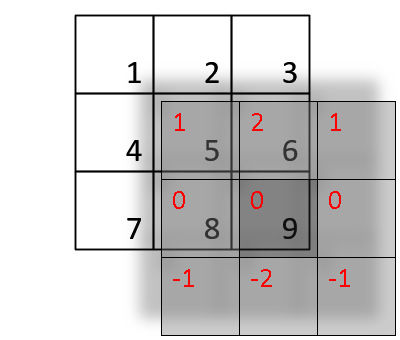
\includegraphics[scale=.2]{figures/mult9.png}
\caption{Exemplo de aplicação de convolução 2D.} \label{gdimotes}
\end{center}
\end{figure}

Nesse trabalho, foram utilizados 2 tipos de filtros:

\begin{enumerate}
	\item Filtro passa-alta: filtros utilizados para realçar certas características presentes nas imagens, tais como bordas, linhas ou regiões de interesse \cite{b2}.
	\item Filtro passa-baixa: filtros utilizados para suavizar as imagens, uma vez que as frequências altas correspondem às transições abruptas são atenuadas \cite{b2}.
\end{enumerate}

Os filtro $h_{1}$, $h_{3}$ e $h_{4}$ são exemplos de filtros passa-alta. Já o filtro $h_{2}$ é um exemplo de filtro passa-baixa. A seguir temos a exemplificação gráfica desses filtros.

\begin{figure}[H]
\begin{center}
	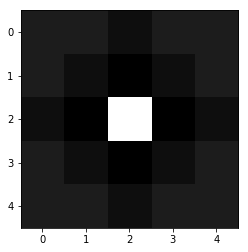
\includegraphics[scale=.3]{figures/h1.png}
	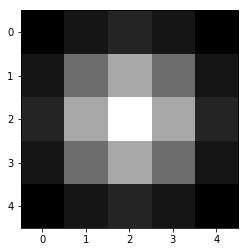
\includegraphics[scale=.3]{figures/h2.png}
\caption{Filtros $h_{1}$ e $h_{2}$.} \label{gdimotes}
\end{center}
\end{figure}

\begin{figure}[H]
\begin{center}
	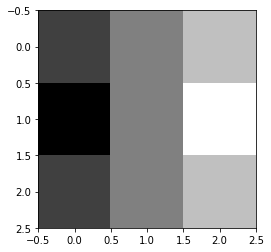
\includegraphics[scale=.3]{figures/h3.png}
	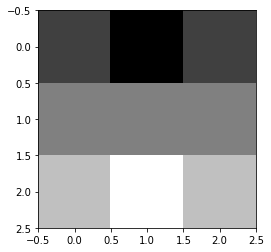
\includegraphics[scale=.3]{figures/h4.png}
\caption{Filtros $h_{3}$ e $h_{4}$.} \label{gdimotes}
\end{center}
\end{figure}

\subsection{Redimensionamento}

A operação de redimensionamento foi utilizada para transformar as saídas da operação de convolução 2D, que não necessariamente estavam no intervalo de escalas de cinza de $\left[0,255\right]$, de volta ao intervalo de escalas de cinza representado por inteiros de 8 \textit{bits}.

\subsection{Transformada Discreta de Fourier}

A Transformada Discreta de Fourier (DFT) é uma transformação de coordenadas em componentes pertencentes ao conjunto dos números complexos, em que cada coeficiente é obtido pela combinação linear dos elementos da entrada com o núcleo da transformada \cite{b2}.

A Transformada de Fourier para duas variáveis pode ser escrita da seguinte forma:

\begin{equation*}
	F(u,v) = \int_{-\infty}^{\infty} \int_{-\infty}^{\infty} f(x,y)exp\left[-j2\pi(ux + vy\right] dx dy
\end{equation*}

e a partir de $F(u,v)$, pode-se obter $f(x,y)$ através da Transformada Inversa de Fourier:

\begin{equation*}
	f(x,y) =  \int_{-\infty}^{\infty} \int_{-\infty}^{\infty} F(u,v)exp\left[j2\pi(ux + vy)\right] du dv.
\end{equation*}

Na filtragem no domínio de frequência, o principal objetivo, é que as operações de convolução possuem o custo computacional menor do que no domínio espacial. Portanto, normalmente, o processamento de imagens possuem a seguinte sequência.

\begin{figure}[H]
\begin{center}
	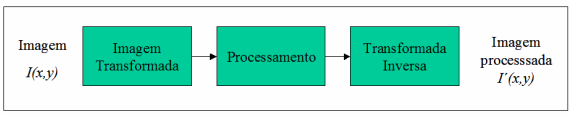
\includegraphics[scale=.35]{figures/sequencia_fourier.png}
\caption{Sequência usualmente utilizada para as operações de processamento de imagens.} \label{gdimotes}
\end{center}
\end{figure}

\subsection{Filtro Gaussiano}

Os filtros Gaussianos são um tipo de filtro passa-baixa, os quais suavizam a imagem filtrada. Nos filtros Gaussianos, os coeficientes da máscara são derivados a partir de uma função Gaussiana bidimensional \cite{b2}. A função Gaussiana discreta com média zero e desvio padrão $\sigma$ é definida como

\begin{equation*}
	G(x,y) = \dfrac{1}{2\pi\sigma^{2}}exp\left(\dfrac{-(x^{2} + y^{2})}{2\sigma^{2}}\right).
\end{equation*}

As variações de sigma utilizados neste trabalho foram: $\sigma = \left[2,4,8,16,32,64\right]$.

\begin{figure}[H]
\begin{center}
	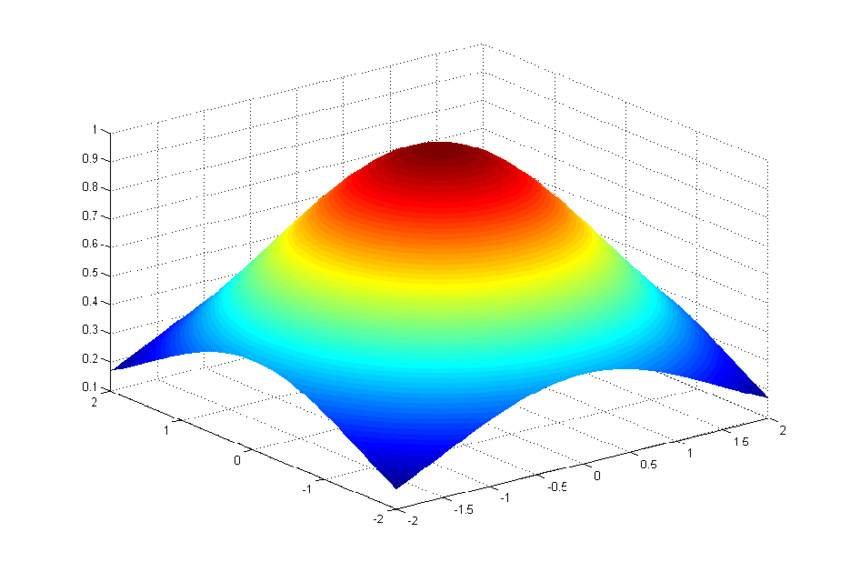
\includegraphics[scale=.2]{figures/filtro_gaussiano.png}
\caption{Exemplificação gráfica de um filtro Gaussiano.} \label{gdimotes}
\end{center}
\end{figure}

%------------------------------------------------

\section{Saída de Dados}

Os imagens resultantes da seção \textbf{1.1} e \textbf{1.2} foram salvas dentro da pasta \textbf{resultados/} utilizando uma função da biblioteca \textbf{matplotlib} chamada \textbf{matplotlib.pyplot.imsave()} \cite{b3}.

O formato dos nomes de saída estão da seguinte forma: para a seção \textbf{1.1} o padrão é o nome da imagem de entrada (\textit{baboon} ou \textit{butterfly}) concatenado com o nome do filtro aplicado sobre ela; na seção \textbf{1.2} são geradas 4 imagens principais resultantes para cada valor de sigma atribuído na função de criar um filtro gaussiano.

%------------------------------------------------

\section{Resultados e Discuções}

Os resultados obtidos na execução dos códigos da \textbf{seção 1.1} estão a seguir:

\begin{figure}[H]
\begin{center}
	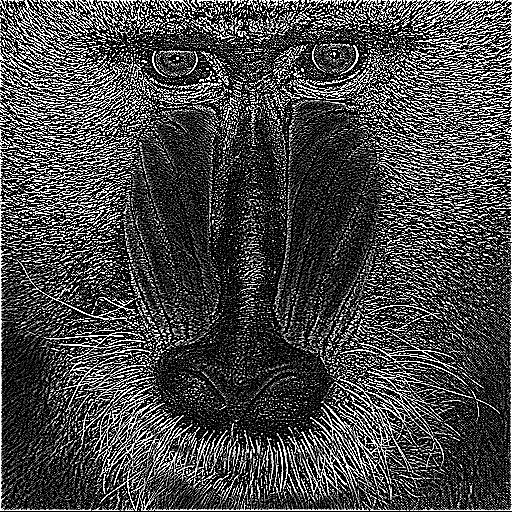
\includegraphics[scale=.19]{figures/baboon_h1.png}
	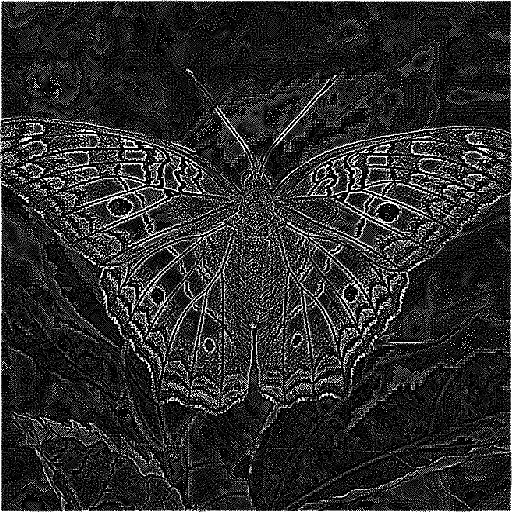
\includegraphics[scale=.19]{figures/butterfly_h1.png}
\caption{Resultado da aplicação do filtro $h_{1}$.} \label{gdimotes}
\end{center}
\end{figure}

Como já dito, o filtro $h_{1}$ é do tipo passa-alta, o qual atenua o valor central da máscara considerada na imagem. Como resultado da passagem desse filtros nas imagens de entrada, podemos observar que os \textit{pixels} de maior intensidade na imagem original foram intensificados, e os \textit{pixels} de menor intensidade tiveram seus valores reduzidos.

\begin{figure}[H]
\begin{center}
	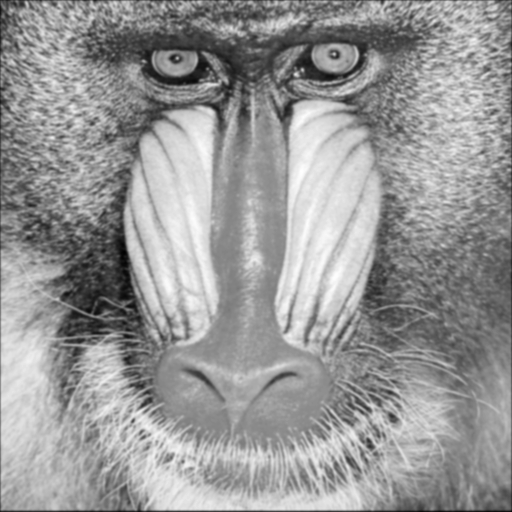
\includegraphics[scale=.19]{figures/baboon_h2.png}
	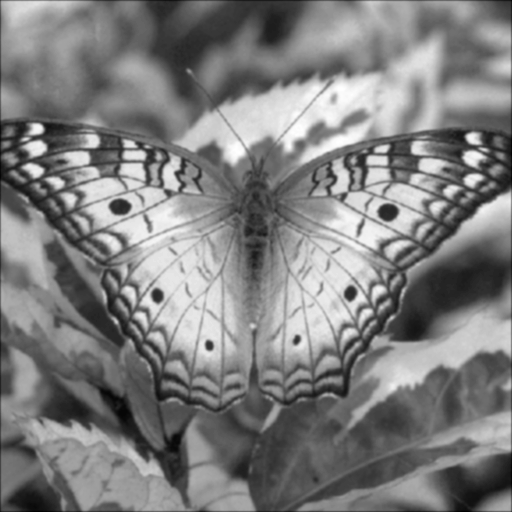
\includegraphics[scale=.19]{figures/butterfly_h2.png}
\caption{Resultado da aplicação do filtro $h_{2}$.} \label{gdimotes}
\end{center}
\end{figure}

O filtro $h_{2}$ é do tipo passa-baixa, pois é baseado em uma distribuição estatística, nesse caso, a média. O resultado obtido pela convolução do filtro $h_{2}$ com as imagens de entrada nos dá como saída imagens suavizadas (com um leve borramento), pois nesse tipo de filtro, os valores de \textit{pixels} da vizinhança são levados em consideração no cálculo do \textit{pixel} central da posição corrente.

\begin{figure}[H]
\begin{center}
	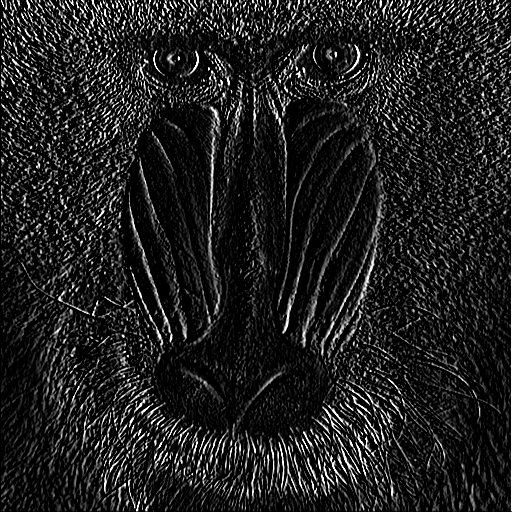
\includegraphics[scale=.19]{figures/baboon_h3.png}
	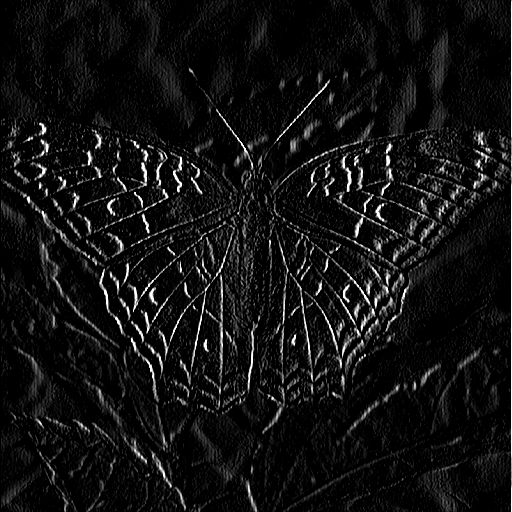
\includegraphics[scale=.19]{figures/butterfly_h3.png}
\caption{Resultado da aplicação do filtro $h_{3}$.} \label{gdimotes}
\end{center}
\end{figure}

O filtro $h_{3}$ é do tipo passa-alta, pois a soma acumulada das células é 0. Esse é um filtro muito conhecido na área de processamento de imagens, denominado \textit{Filtro de Sobel}. A aplicação desse filtro consiste num operador que calcula diferenças finitas, dando uma aproximação do gradiente da intensidade dos \textit{pixels} da imagem. Como resultado da aplicação do filtro $h_{3}$ temos a detecção de bordas na vertical nas imagens de entrada.

\begin{figure}[H]
\begin{center}
	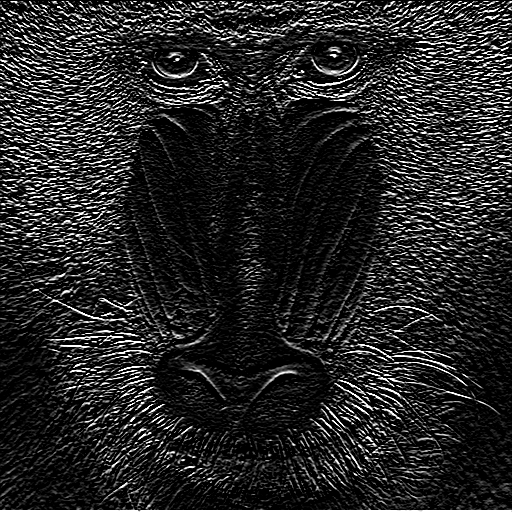
\includegraphics[scale=.19]{figures/baboon_h4.png}
	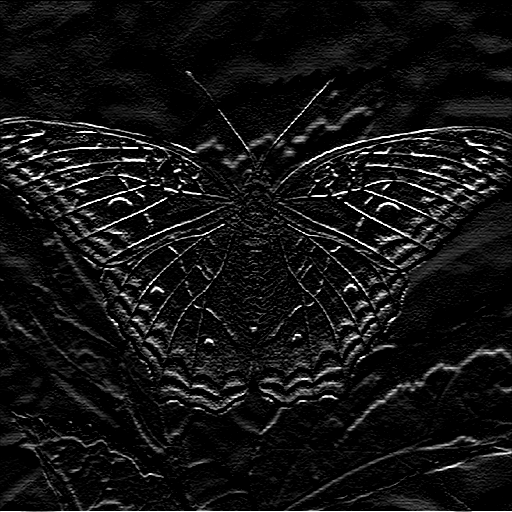
\includegraphics[scale=.19]{figures/butterfly_h4.png}
\caption{Resultado da aplicação do filtro $h_{4}$.} \label{gdimotes}
\end{center}
\end{figure}

O filtro $h_{4}$ também é do tipo passa-alta e também é denominado como \textit{Filtro de Sobel}. Porém, esse filtro detecta bordas na horizontal em imagens, atenuando esse valores para que passem a ficar mais visíveis na imagem de saída.

\begin{figure}[H]
\begin{center}
	
\includegraphics[scale=.19]{figures/baboon_h.png}
	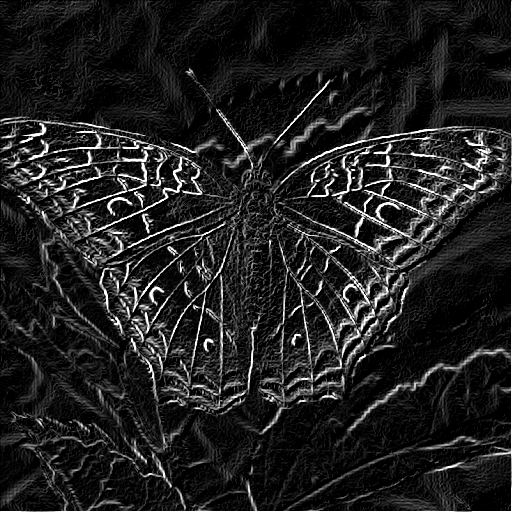
\includegraphics[scale=.19]{figures/butterfly_h.png}
\caption{Resultado da expressão $\sqrt{(h_{3})^{2} + (h_{4})^{2}}$.} \label{gdimotes}
\end{center}
\end{figure}

Como resultado da combinação, somando-se as respostas de cada um filtros por meio da expressão $\sqrt{(h_{3})^{2} + (h_{4})^{2}}$ temos uma imagem que equilibra a detecção de bordas na vertical, obtidas com a aplicação do filtro $h_{3}$, e a detecção de bordas na horizontal, obtidas com a aplicação do filtro $h_{4}$. Os componentes que estão elevados ao quadrado tem como objetivo a atenuação das componentes de alta intensidade, assim, com a operação de radiciação, obtemos um grau de combinação entre as linhas verticais e horizontais.

Os resultados obtidos na execução dos códigos da \textbf{seção 1.2} estão a seguir:

\begin{figure}[H]
\begin{center}
	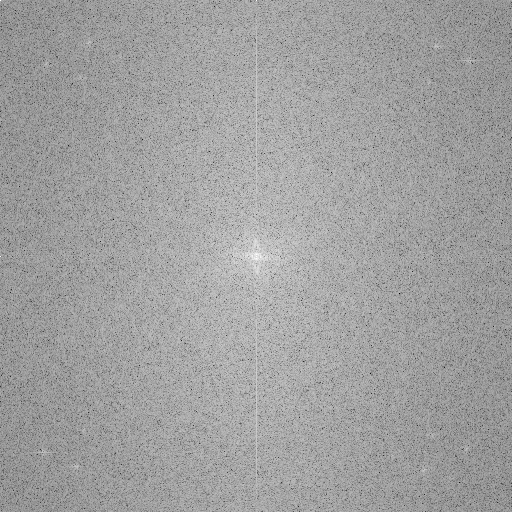
\includegraphics[scale=.17]{figures/baboon_mag_spec_4.png}
	
\includegraphics[scale=.17]{figures/baboon_gau_filter_4.png}
	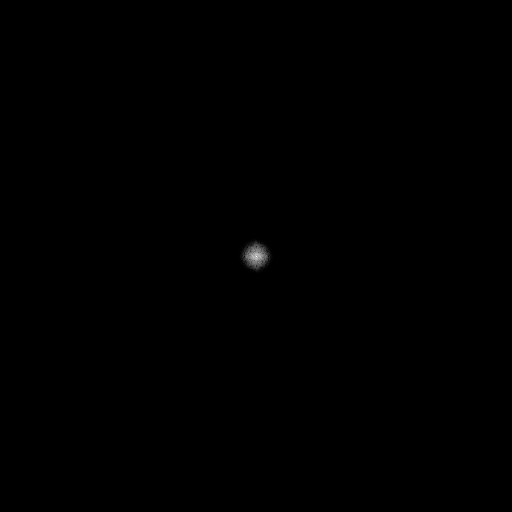
\includegraphics[scale=.17]{figures/baboon_mag_filter_4.png}
	
\includegraphics[scale=.17]{figures/baboon_result_4.png}
\caption{Resultados obtidos com o sigma valendo 4.} \label{mag_4}
\end{center}
\end{figure}

Na Figura~\ref{mag_4} temos, na primeira imagem, o espectro de magnitude gerado após a aplicação da \textit{Transformada Discreta de Fourier} na imagem e a componente de frequência zero ser transladada para o centro da imagem. Na segunda imagem da primeira linha temos a visualização gráfica de um filtro gaussiano com média 0 e desvio padrão de valor 4, como o filtro é do tamanho da imagem, os intensidades visíveis estão agrupadas em um circulo bem pequeno no centro da imagem, por conta do baixo valor de desvio padrão. Na primeira imagem da segunda linha temos o resultado da aplicação do filtro gaussiano no espectro de frequência da imagem \textit{baboon.png}. Como o filtro em questão possui um baixo valor de desvio padrão, então ao ser aplicado pelo espectro de frequência, ele deixa passar somente valores correspondentes a sua área. Nesse caso, o espectro de frequência resultante perdeu informações sobre as frequências mais altas (que são as componentes presentes em regiões mais escuras). Por fim, a segunda imagem da segunda linha é o resultado da aplicação da \textit{Transformada Inversa de Fourier}, que transforma a imagem de volta para o domínio espacial. Podemos observar que, como houve a aplicação de um filtro gaussiano com baixo desvio padrão, a imagem resultante possui um borramento alto em comparação com a imagem original.

\begin{figure}[H]
\begin{center}
	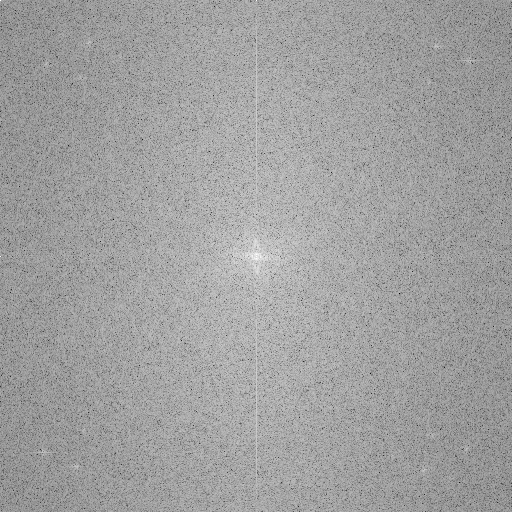
\includegraphics[scale=.17]{figures/baboon_mag_spec_32.png}
	
\includegraphics[scale=.17]{figures/baboon_gau_filter_32.png}
	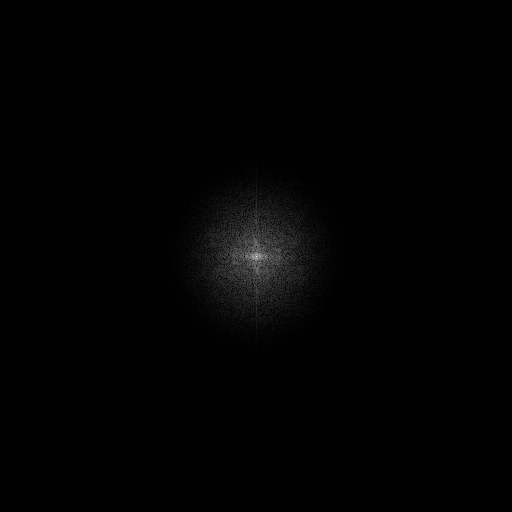
\includegraphics[scale=.17]{figures/baboon_mag_filter_32.png}
	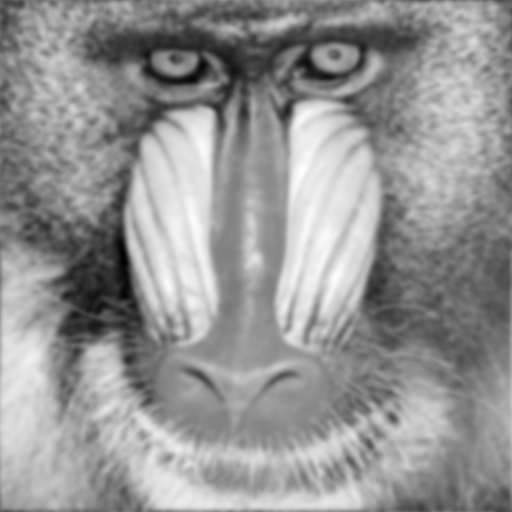
\includegraphics[scale=.17]{figures/baboon_result_32.png}
\caption{Resultados obtidos com o sigma valendo 32.} \label{mag_32}
\end{center}
\end{figure}

Na Figura~\ref{mag_32} temos a mesma ordem da figura anterior, porém, nesse caso, o valor de desvio padrão aplicado foi de 32. Podemos ver que o filtro possui uma circunferência bem maior e que, assim, após a aplicação desse filtro no espectro de frequência da imagem original, o espectro de frequência resultante possui mais componentes de frequências mais altas do que a anterior. Portanto, após a aplicação da função inversa, vemos que a imagem resultante possui somente um leve borramento, pois seu espectro tinha mais informações.

\begin{figure}[H]
\begin{center}
	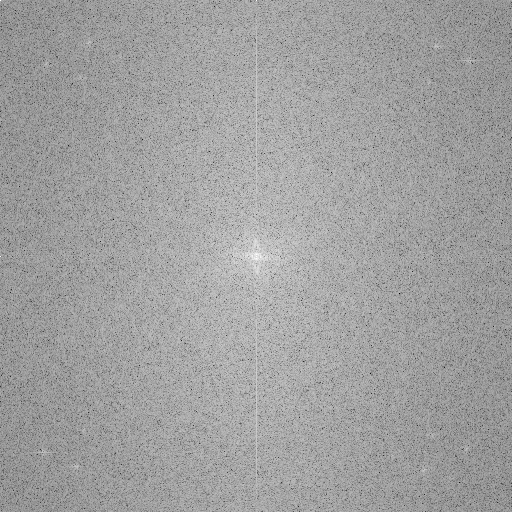
\includegraphics[scale=.17]{figures/baboon_mag_spec_64.png}
	
\includegraphics[scale=.17]{figures/baboon_gau_filter_64.png}
	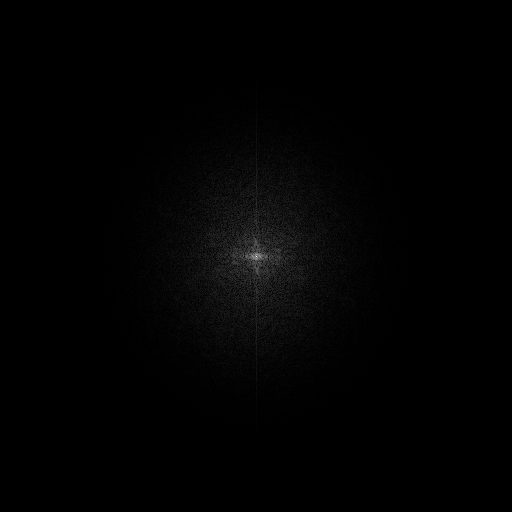
\includegraphics[scale=.17]{figures/baboon_mag_filter_64.png}
	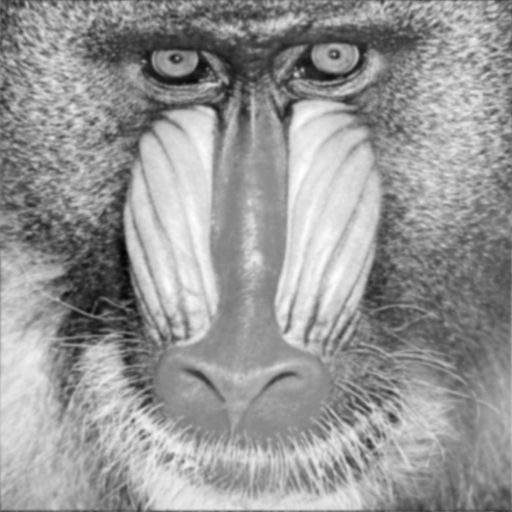
\includegraphics[scale=.17]{figures/baboon_result_64.png}
\caption{Resultados obtidos com o sigma valendo 64.} \label{mag_64}
\end{center}
\end{figure}

Por fim, na Figura~\ref{mag_64} temos um filtro gaussiano com desvio padrão valendo 64. Podemos observar que o filtro ficou bem mais abrangente, em relação aos anteriores, e que sua aplicação no espectro de frequência deixou passar componentes de frequências bem mais altas, que resultam em mais informações para a reconstrução da imagem inicial. Como resultado final, vemos que a imagem possui um grau de detalhes bem maior que os resultados anteriores e que já é bem mais próxima da imagem original.

Portanto, com esses resultados podemos observar que quanto maior o filtro gaussiano, mais informações do espectro de frequência vão ser liberados e, assim, na aplicação da \textit{Transformação Inversa de Fourier}, a função terá bem mais informações para a resconstrução da imagem original. Quanto mais informações no espectro de frequência resultante, mais próximo da imagem original é o resultante e, analogamente, quanto menos informações no espectro de frequência resultante, mais distante (mais borrado) da imagem original é o resultado.

%------------------------------------------------

\section{Conclusão}

Podemos concluir que os resultados obtidos na \textbf{seção 1.1} e na \textbf{seção 1.2} foram satisfatórios quanto a especificação do trabalho e que a visualização prática dos tipos de filtros (passa-alta e passa-baixa), aplicação de filtros no domínio de frequência, mudanças de domínios das imagens e combinação de resultados, consolida ainda mais os conceitos vistos em sala de aula.

%----------------------------------------------------------------------------------------
%	REFERENCE LIST
%----------------------------------------------------------------------------------------

\begin{thebibliography}{99} % Bibliography - this is intentionally simple in this template

\bibitem{b1} Welcome to opencv documentation! \href{https://docs.opencv.org/2.4/index.html}{https://docs.opencv.org/2.4/index.html} Acesso em: 15/04/2019.

\bibitem{b2} Pedrini, Hélio, and William Robson Schwartz. Análise de imagens digitais: princípios, algoritmos e aplicações. Thomson Learning, 2008.

\bibitem{b3} Matplotlib Version 3.0.3 \href{https://matplotlib.org/contents.html}{https://matplotlib.org/contents.html} Acesso em: 15/04/2019.
 
\end{thebibliography}

%----------------------------------------------------------------------------------------

\section*{Anexos}

\begin{figure}[H]
\begin{center}
	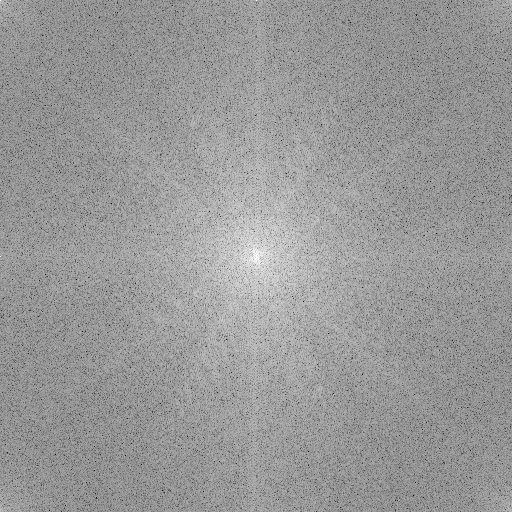
\includegraphics[scale=.19]{figures/butterfly_mag_spec_2.png}
	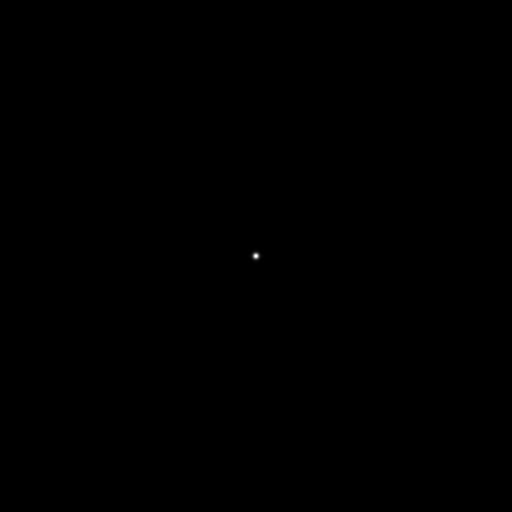
\includegraphics[scale=.19]{figures/butterfly_gau_filter_2.png}
	
\includegraphics[scale=.19]{figures/butterfly_mag_filter_2.png}
	
\includegraphics[scale=.19]{figures/butterfly_result_2.png}
\caption{Resultados obtidos com o sigma valendo 2.} \label{mag_64}
\end{center}
\end{figure}

\begin{figure}[H]
\begin{center}
	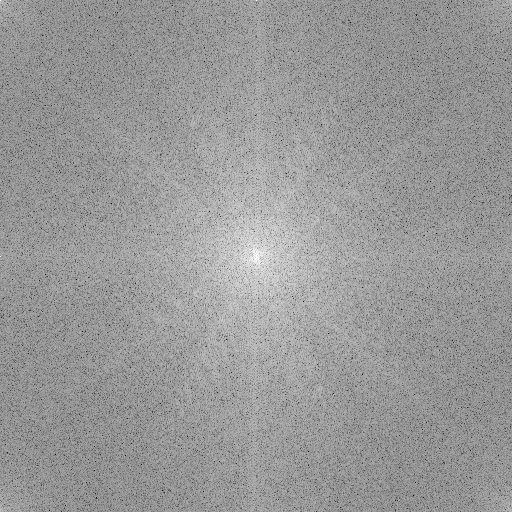
\includegraphics[scale=.19]{figures/butterfly_mag_spec_4.png}
	
\includegraphics[scale=.19]{figures/butterfly_gau_filter_4.png}
	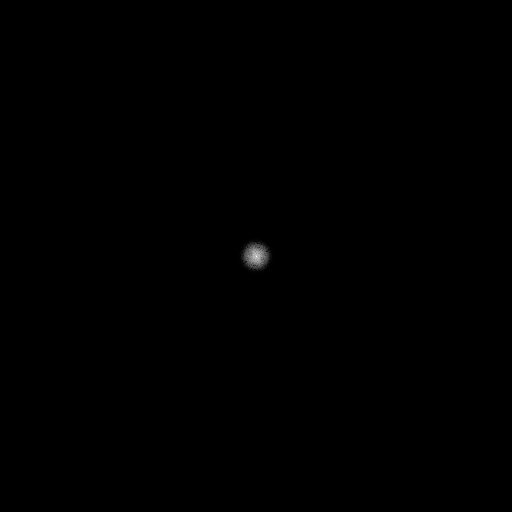
\includegraphics[scale=.19]{figures/butterfly_mag_filter_4.png}
	
\includegraphics[scale=.19]{figures/butterfly_result_4.png}
\caption{Resultados obtidos com o sigma valendo 4.} \label{mag_64}
\end{center}
\end{figure}

\begin{figure}[H]
\begin{center}
	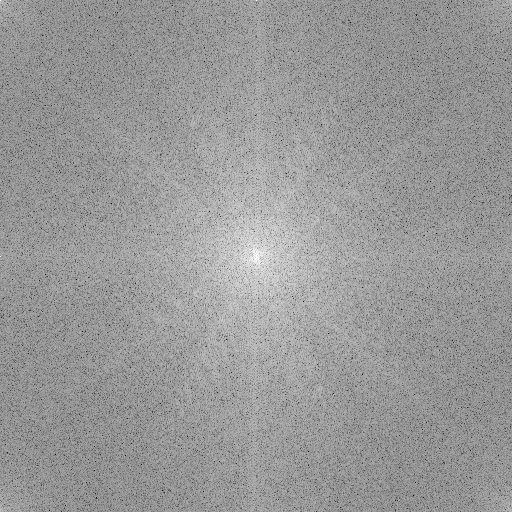
\includegraphics[scale=.19]{figures/butterfly_mag_spec_8.png}
	
\includegraphics[scale=.19]{figures/butterfly_gau_filter_8.png}
	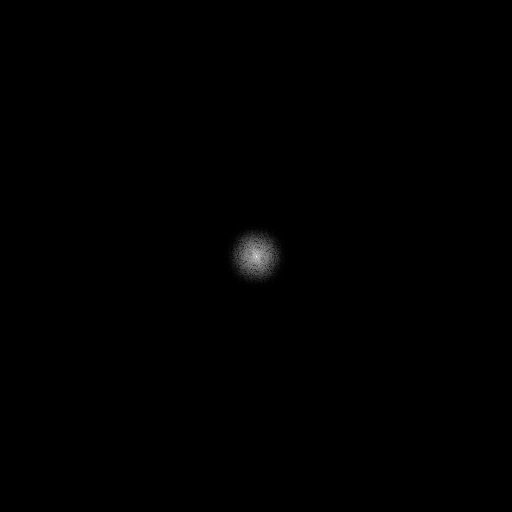
\includegraphics[scale=.19]{figures/butterfly_mag_filter_8.png}
	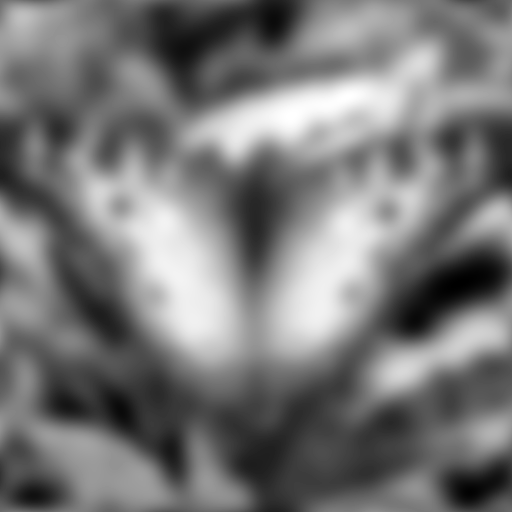
\includegraphics[scale=.19]{figures/butterfly_result_8.png}
\caption{Resultados obtidos com o sigma valendo 8.} \label{mag_64}
\end{center}
\end{figure}

\begin{figure}[H]
\begin{center}
	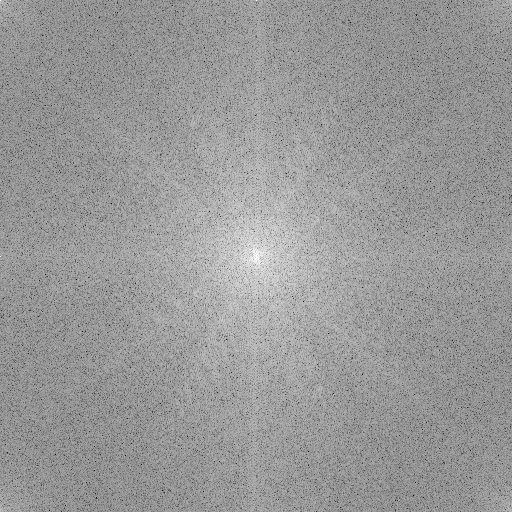
\includegraphics[scale=.19]{figures/butterfly_mag_spec_16.png}
	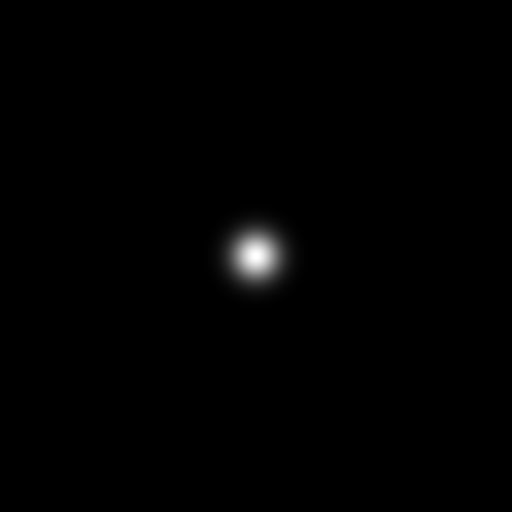
\includegraphics[scale=.19]{figures/butterfly_gau_filter_16.png}
	\includegraphics[scale=.19]{figures/butterfly_mag_filter_16.png}
	\includegraphics[scale=.19]{figures/butterfly_result_16.png}
\caption{Resultados obtidos com o sigma valendo 16.} \label{mag_64}
\end{center}
\end{figure}

\begin{figure}[H]
\begin{center}
	\includegraphics[scale=.19]{figures/butterfly_mag_spec_32.png}
	\includegraphics[scale=.19]{figures/butterfly_gau_filter_32.png}
	\includegraphics[scale=.19]{figures/butterfly_mag_filter_32.png}
	\includegraphics[scale=.19]{figures/butterfly_result_32.png}
\caption{Resultados obtidos com o sigma valendo 32.} \label{mag_64}
\end{center}
\end{figure}

\begin{figure}[H]
\begin{center}
	\includegraphics[scale=.19]{figures/butterfly_mag_spec_64.png}
	\includegraphics[scale=.19]{figures/butterfly_gau_filter_64.png}
	\includegraphics[scale=.19]{figures/butterfly_mag_filter_64.png}
	\includegraphics[scale=.19]{figures/butterfly_result_64.png}
\caption{Resultados obtidos com o sigma valendo 64.} \label{mag_64}
\end{center}
\end{figure}

\end{document}
